\documentclass{article}

\usepackage{graphicx} % Required for inserting images
\usepackage[left=1in,right=1in,top=1in,bottom=1in]{geometry}
\usepackage{amsmath}
\usepackage{amsthm} %proof environment
\usepackage{amssymb}
\usepackage{amsfonts}
\usepackage{enumitem} %nice lists
\usepackage{verbatim} %useful for something 
\usepackage{xcolor}
\usepackage{setspace}
\usepackage{blindtext} % I have no idea what this is 
\usepackage{caption}  % need this for unnumbered captions/figures
\usepackage{natbib}
\usepackage{tikz}
\usepackage{soul} % need this for the hl command
\usepackage{hyperref}

\begin{document}

\title{Midterm 2 - AM 212}
\author{Dante Buhl}
\date{November 26, 2024}


\newcommand{\wrms}{w_{\text{rms}}}
\newcommand{\bs}[1]{\boldsymbol{#1}}
\newcommand{\tb}[1]{\textbf{#1}}
\newcommand{\bmp}[1]{\begin{minipage}{#1\textwidth}}
\newcommand{\emp}{\end{minipage}}
\newcommand{\R}{\mathbb{R}}
\newcommand{\C}{\mathbb{C}}
\newcommand{\N}{\mathcal{N}}
\newcommand{\K}{\bs{\mathrm{K}}}
\newcommand{\m}{\bs{\mu}_*}
\newcommand{\s}{\bs{\Sigma}_*}
\newcommand{\dt}{\Delta t}
\newcommand{\dx}{\Delta x}
\newcommand{\tr}[1]{\text{Tr}(#1)}
\newcommand{\Tr}[1]{\text{Tr}(#1)}
\newcommand{\Div}{\nabla \cdot}
\renewcommand{\div}{\nabla \cdot}
\newcommand{\Curl}{\nabla \times}
\newcommand{\Grad}{\nabla}
\newcommand{\grad}{\nabla}
\newcommand{\grads}{\nabla_s}
\newcommand{\gradf}{\nabla_f}
\newcommand{\xs}{x_s}
\newcommand{\xf}{x_f}
\newcommand{\ts}{t_s}
\newcommand{\tf}{t_f}
\newcommand{\pt}{\partial t}
\newcommand{\pz}{\partial z}
\newcommand{\uvec}{\bs{u}}
\newcommand{\F}{\bs{F}}
\newcommand{\T}{\tilde{T}}
\newcommand{\ez}{\bs{e}_z}
\newcommand{\ex}{\bs{e}_x}
\newcommand{\ey}{\bs{e}_y}
\newcommand{\eo}{\bs{e}_{\bs{\Omega}}}
\newcommand{\ppt}[1]{\frac{\partial #1}{\partial t}}
\newcommand{\ppts}[1]{\frac{\partial #1}{\partial t_s}}
\newcommand{\pptf}[1]{\frac{\partial #1}{\partial t_f}}
\newcommand{\ppz}[1]{\frac{\partial #1}{\partial z}}
\newcommand{\ddz}[1]{\frac{d #1}{d z}}
\newcommand{\ppzetas}[1]{\frac{\partial^2 #1}{\partial \zeta^2}}
\newcommand{\ppzs}[1]{\frac{\partial #1}{\partial z_s}}
\newcommand{\ppzf}[1]{\frac{\partial #1}{\partial z_f}}
\newcommand{\ppx}[1]{\frac{\partial #1}{\partial x}}
\newcommand{\ppy}[1]{\frac{\partial #1}{\partial y}}
\newcommand{\ppzeta}[1]{\frac{\partial #1}{\partial \zeta}}


\maketitle 

\section*{Problem 1}
For each of the following 3 ODEs,
\begin{enumerate}[label=\alph*.]
    \item Plot the numerical solution for $\epsilon = 0.1$, $\epsilon = 0.01$,
    and $\epsilon = 0.001$
    \item Explain in a few words of what method you plan to use the solve this
    asymptotically and why, based on the numerical solution
    \item Find the lowest order uniformly convergent analytical approximation to
    the solution for small positive $\epsilon$. 
    \item Compare the numerical and analytical solutions for $\epsilon = 0.01$. 
\end{enumerate}

\vspace{20pt}

ODE A: 

\begin{gather*}
    \frac{d^2f}{dt^2} = -f - \epsilon f^2 \left(\frac{df}{dt}\right) \quad
    \text{with } f(0) = 1, \frac{df}{dt}(0) = 0
\end{gather*}

\begin{enumerate}[label=\alph*.]
    \item See Figure \ref{fig:ODEA_num_sol}
        \begin{figure}[ht]
            \centering
            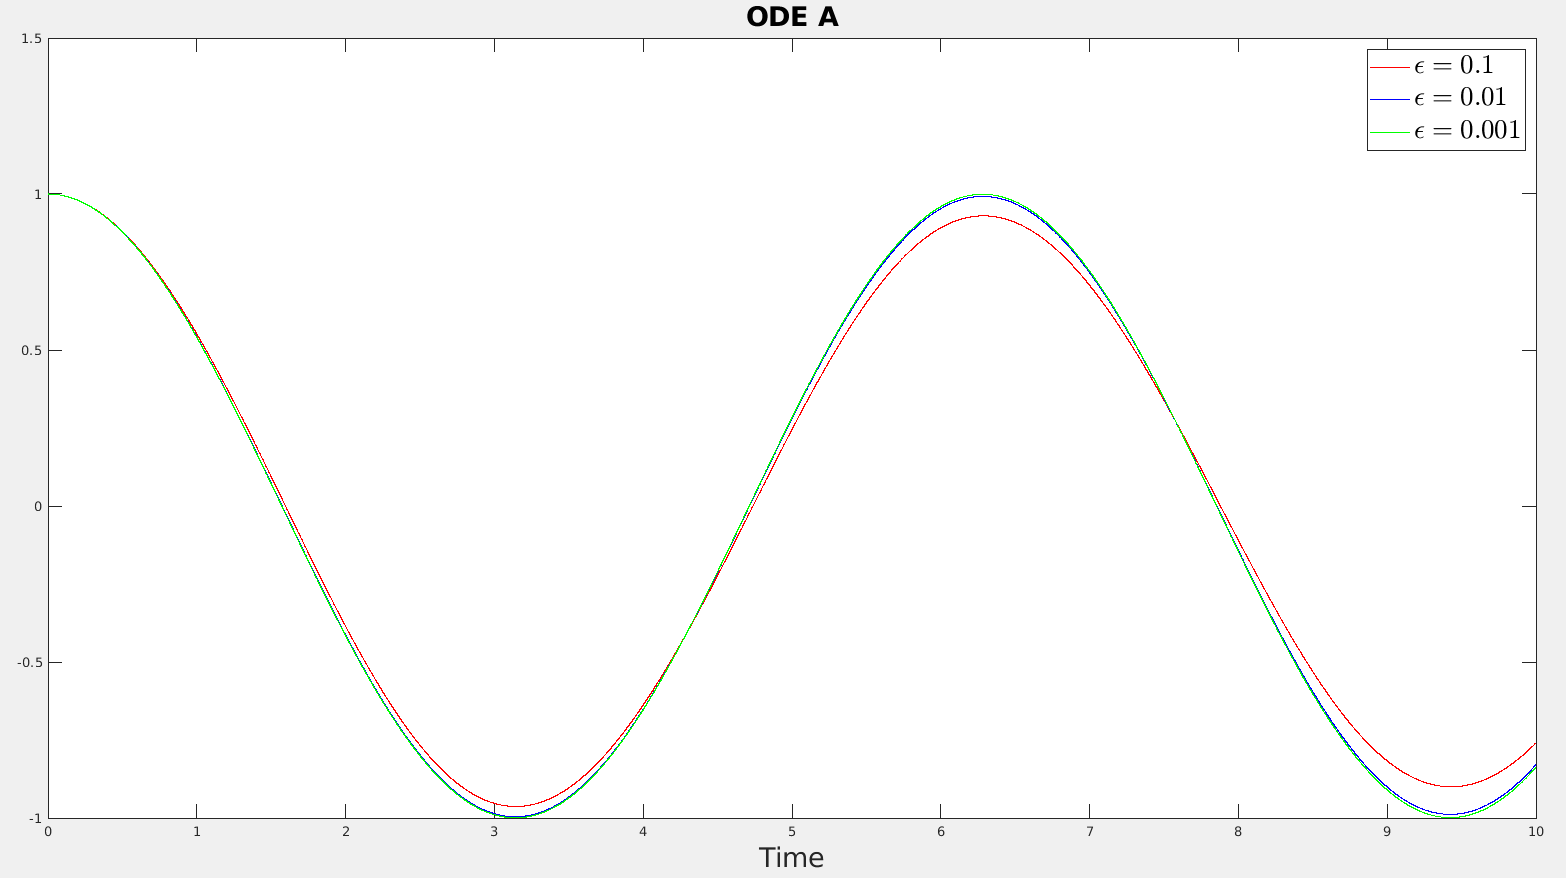
\includegraphics[width=.8\textwidth]{images/ODEA.png}
            \caption{Numerical Solution for differing $\epsilon$ using `ode45'}
            \label{fig:ODEA_num_sol}
        \end{figure}
    \item For this problem, we will use the multiscale method as it seems that
    the amplitude of the sine wave seems to decay on a timescale which is
    dependent on epsilon (on a longer time series it is clear that all three
    solutions decay). 
    \item To find the lowest order solution we first begin with the multiscale
    method. 
    \begin{gather*}
        \ts = \epsilon t, \quad \tf =  t\\
        \ppts{} = \frac{dt}{d\ts}\ppt{}, \quad \pptf{} = \ppt{}
    \end{gather*}
    \begin{gather*}
        \left(\epsilon\ppts{} + \pptf{}\right)\left(\epsilon\ppts{} + \pptf{}\right)[f_0
        +\epsilon f_1 + \cdots] =\\
        -(f_0 +\epsilon f_1 + \cdots) -
        \epsilon (f_0 + \epsilon f_1 + \cdots)^2\left(\epsilon \ppts{} +
        \pptf{}\right)[f_0 + \epsilon f_1 + \cdots]\\
        f_0 (0) = 1, \quad f_i(0) = 0, \enspace \forall i \ge 1, \quad \ppt{f_i} =
        0, \enspace
        \forall i \ge 0
    \end{gather*}
    \begin{gather*}
        O(\epsilon^0): \quad \frac{\partial^2f_0}{\partial \tf^2} = -f_0
        \implies f_0 = cos(\tf)g(\ts)\\
        O(\epsilon): \quad \frac{\partial^2f_1}{\partial \tf^2}
        -2\ppts{g}\sin(\tf) = -f_1 + \cos^2(\tf)\sin(\tf)g^3(\ts)
    \end{gather*}
    The term $\cos^2(\tf)\sin(\tf)$ in the $O(\epsilon)$ equation produces a
    secular term. Using some trig identities we find that thie reduces to:
    \begin{gather*}
        \cos^2(\tf)\sin(\tf) = \frac{1}{4}\sin(\tf) + \frac{1}{4}\sin(3\tf)
    \end{gather*}
    We solve for $g(\ts)$ in order to eliminate this secular term. (Notice that
    a partial derivative in this case becomes a regular derivative since g only
    depends on $\ts$). 
    \begin{gather*}
        -2\frac{dg}{d\ts}\sin(\tf) = \frac{1}{4}\sin(\tf)g^3(\ts)\\
        \frac{dg}{g^3} = -\frac{d\ts}{8}\\
        -\frac{1}{2g^2} = -\frac{\ts}{8} + c\\
        g = \left(\frac{\ts}{4} + c\right)^{-1/2}\\
        g = \left(\frac{\ts}{4} + 1\right)^{-1/2}, \quad \textbf{IC}\\
        f_0 = \left(\frac{\ts}{4} + 1\right)^{-1/2}\sin(\tf)
    \end{gather*}
    This choice of $f_0$ successfully eliminates the secular term allowing $f_1$
    to be bounded and therefore producing a uniform expansion. Thus the lowest
    order solution needed is $O(1)$. 
    \item The numerical and asymptotic solutions align very nicely for this
    problem (see Figure \ref{fig:ODEA_comp}). Although the solution for
    $\epsilon = 0.01$ decays very slowly, its decline is visible within 50 time
    units. 
        \begin{figure}[ht]
            \centering
            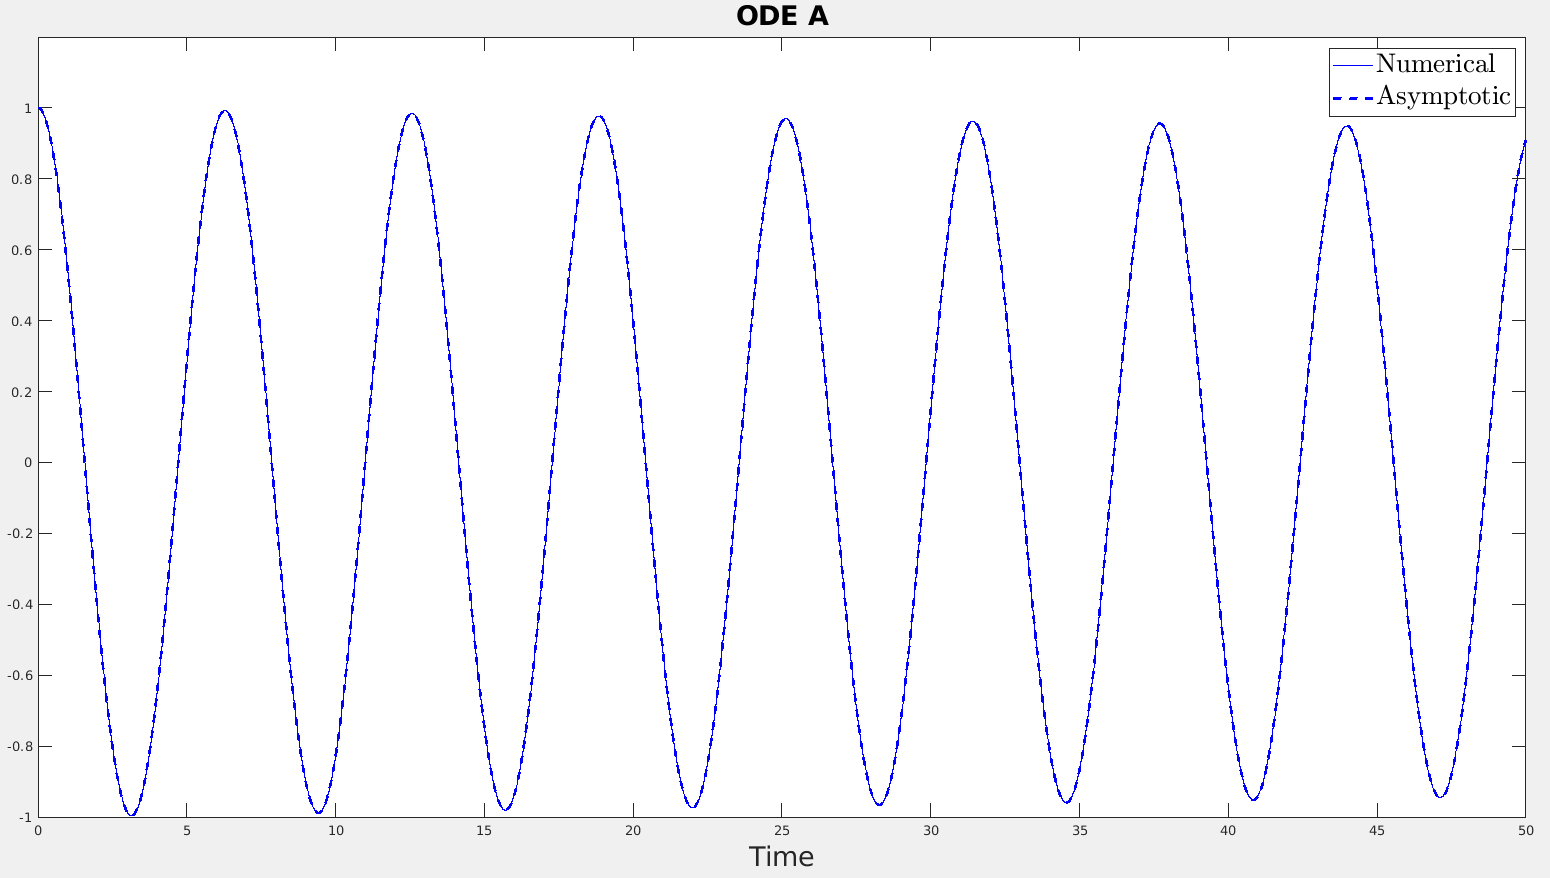
\includegraphics[width=.8\textwidth]{images/ODEA_sol.png}
            \caption{Comparison between numerical and asymptotic solutions for
            $\epsilon = 0.01$}
            \label{fig:ODEA_comp}
        \end{figure}
    
\end{enumerate}

\vspace{20pt}

ODE B: 

\begin{gather*}
    \frac{d^2f}{dt^2} = -f - \epsilon f \left(\frac{df}{dt}\right)^4 \quad
    \text{with } f(0) = 1, \frac{df}{dt}(0) = 0
\end{gather*}

\begin{enumerate}[label=\alph*.]
    \item See Figure \ref{fig:ODEB_num_sol}
        \begin{figure}[ht]
            \centering
            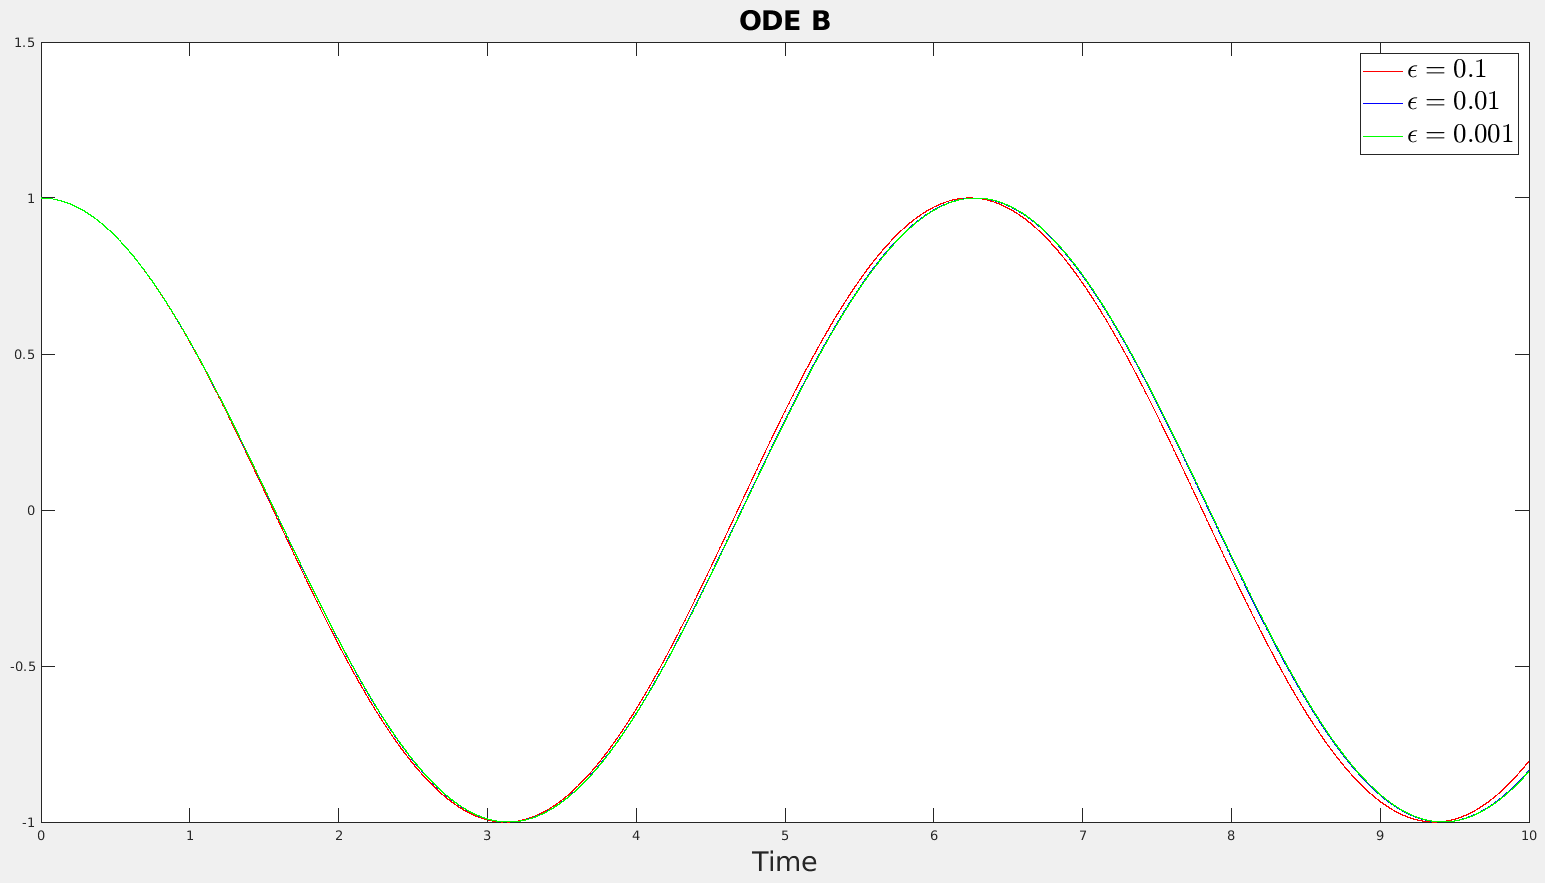
\includegraphics[width=.8\textwidth]{images/ODEB.png}
            \caption{Numerical Solution for differing $\epsilon$ using `ode45'}
            \label{fig:ODEB_num_sol}
        \end{figure}
    \item I will solve this problem using the method of strained coordinates
    since the numerical solution suggests that $\epsilon$ will affect the
    periodicity of the solution rather than the amplitude. 
    \item In order to solve this problem we introduce $\tau = t + \epsilon w_1 t
    + O(\epsilon^2)$. We substitute this into the ODE,
    \begin{gather*}
        \frac{d}{dt} = (1 + \epsilon w_1 + O(\epsilon^2))\frac{d}{d\tau}\\
        (1 + 2\epsilon w_1 + \epsilon^2(w_1 + 2w_2) +
        O(\epsilon^3))\frac{d^2f}{d\tau^2} = \\- (f_0 + \epsilon f_1 +
        O(\epsilon^2) - \epsilon (f_0 + \epsilon f_1 + O(\epsilon^2))(1 +
        \epsilon w_1 + O(\epsilon^2))^4\left(\frac{d}{d\tau}(f_0 + \epsilon f_1
        + O(\epsilon^2))\right)\\
        f_0(0) = 1, \quad f_i(0) = 0 \enspace \forall i \ge 1,\quad
        \frac{df_i}{d\tau} = 0 \enspace \forall i
        \ge 0\\
        O(\epsilon^0): \quad \frac{d^2f_0}{d\tau^2} = -f_0 \implies f_0 =
        \cos(\tau)\\
        O(\epsilon^1): \quad \frac{d^2f_1}{d\tau^2} + w_1\frac{df_0}{d\tau}=
        -f_1 - \epsilon f_0f_0'^4 \\
        O(\epsilon^1): \quad \frac{d^2f_1}{d\tau^2} - 2w_1\cos(\tau) =
        -f_1 - \epsilon \cos(\tau)\sin^4(\tau)
    \end{gather*}
    Here the term $\cos(\tau)\sin^4(\tau)$ will produce a secular term causing
    non-uniformity. In order to eliminate the secular term we use a trig
    identity and then fix $w_1$ in order to eliminate this term. 
    \begin{gather*}
        \cos(\tau)\sin^4(\tau) = \frac{1}{8}\cos(\tau) - \frac{3}{16}\cos(3\tau) +
        \frac{1}{16}\cos(5\tau)\\
        -2w_1\cos(\tau) = -\frac{1}{8}\cos(\tau) \implies w_1 = \frac{1}{16}\\
        \tau = t + \frac{\epsilon}{16}t + O(\epsilon^2)
    \end{gather*}
    We have now found $\tau$ to order $\epsilon$ in such a way that $f_1$ is
    bounded and therefore the first order expansion is uniform. 
    \begin{gather*}
        f_0 = \cos\left(t + \frac{\epsilon t}{16}\right)
    \end{gather*} 
    \item As seen in Figure \ref{fig:ODEB_comp}, the asymptotic solution follows
    the numerical solution. 
        \begin{figure}
            \centering
            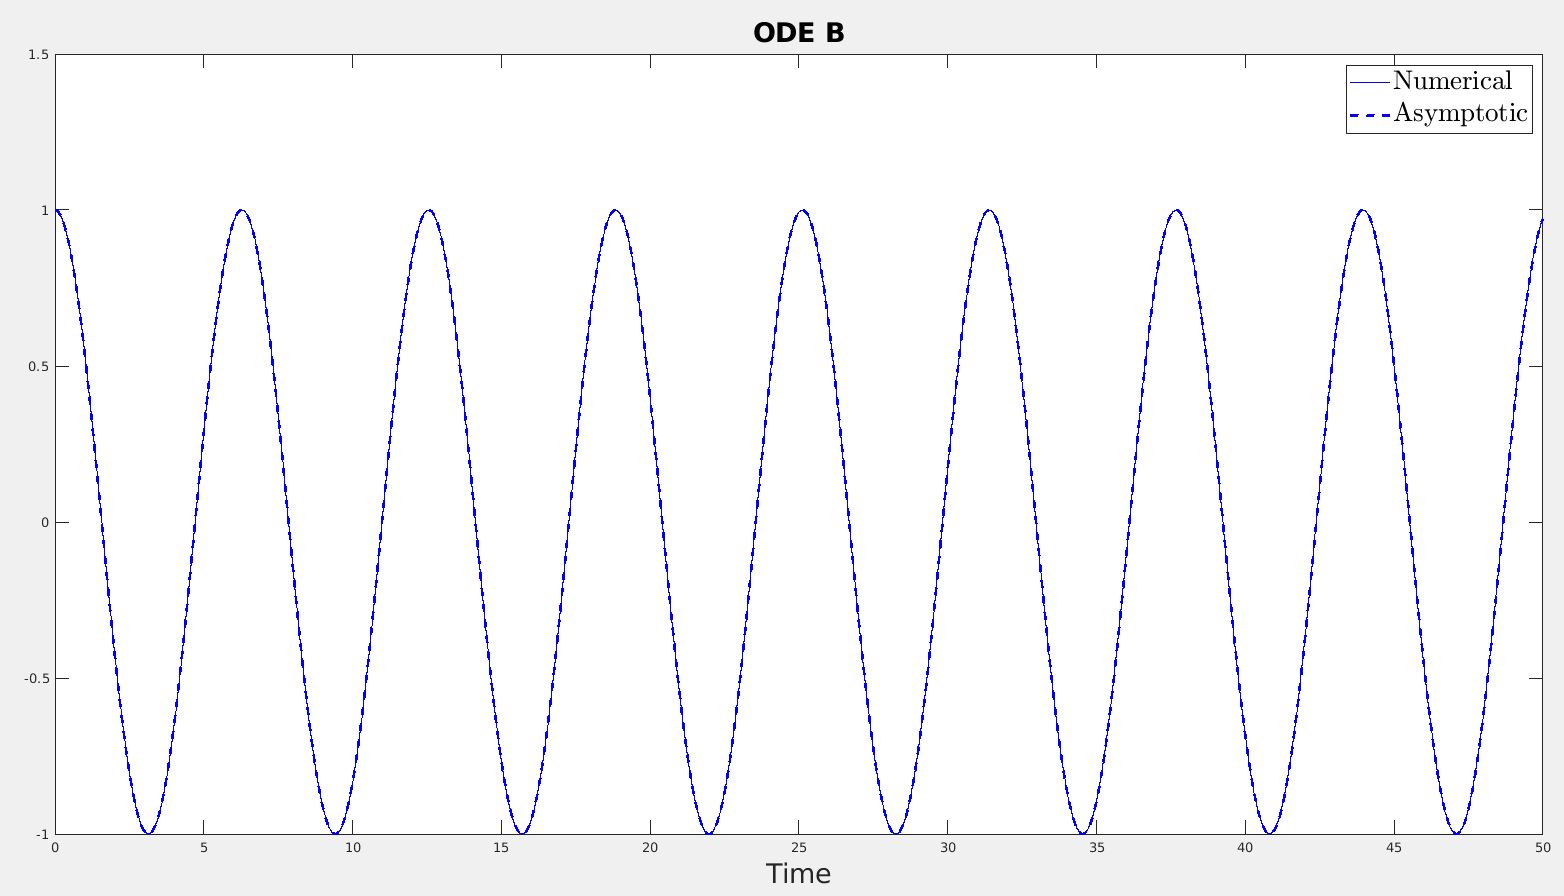
\includegraphics[width=.8\textwidth]{images/ODEB_sol.png}
            \caption{Comparison between numerical and asymptotic solutions for
            $\epsilon = 0.01$}
            \label{fig:ODEB_comp}
        \end{figure}

\end{enumerate}

\vspace{20pt}

ODE C: 

\begin{gather*}
    \epsilon\frac{d^2f}{dt^2} + \frac{df}{dt} + (t+1)f = 0 \quad
    \text{with } f(0) = 1, f(1) = 2
\end{gather*}

\begin{enumerate}[label=\alph*.]
    \item See Figure \ref{fig:ODEC_num_sol}
        \begin{figure}[ht]
            \centering
            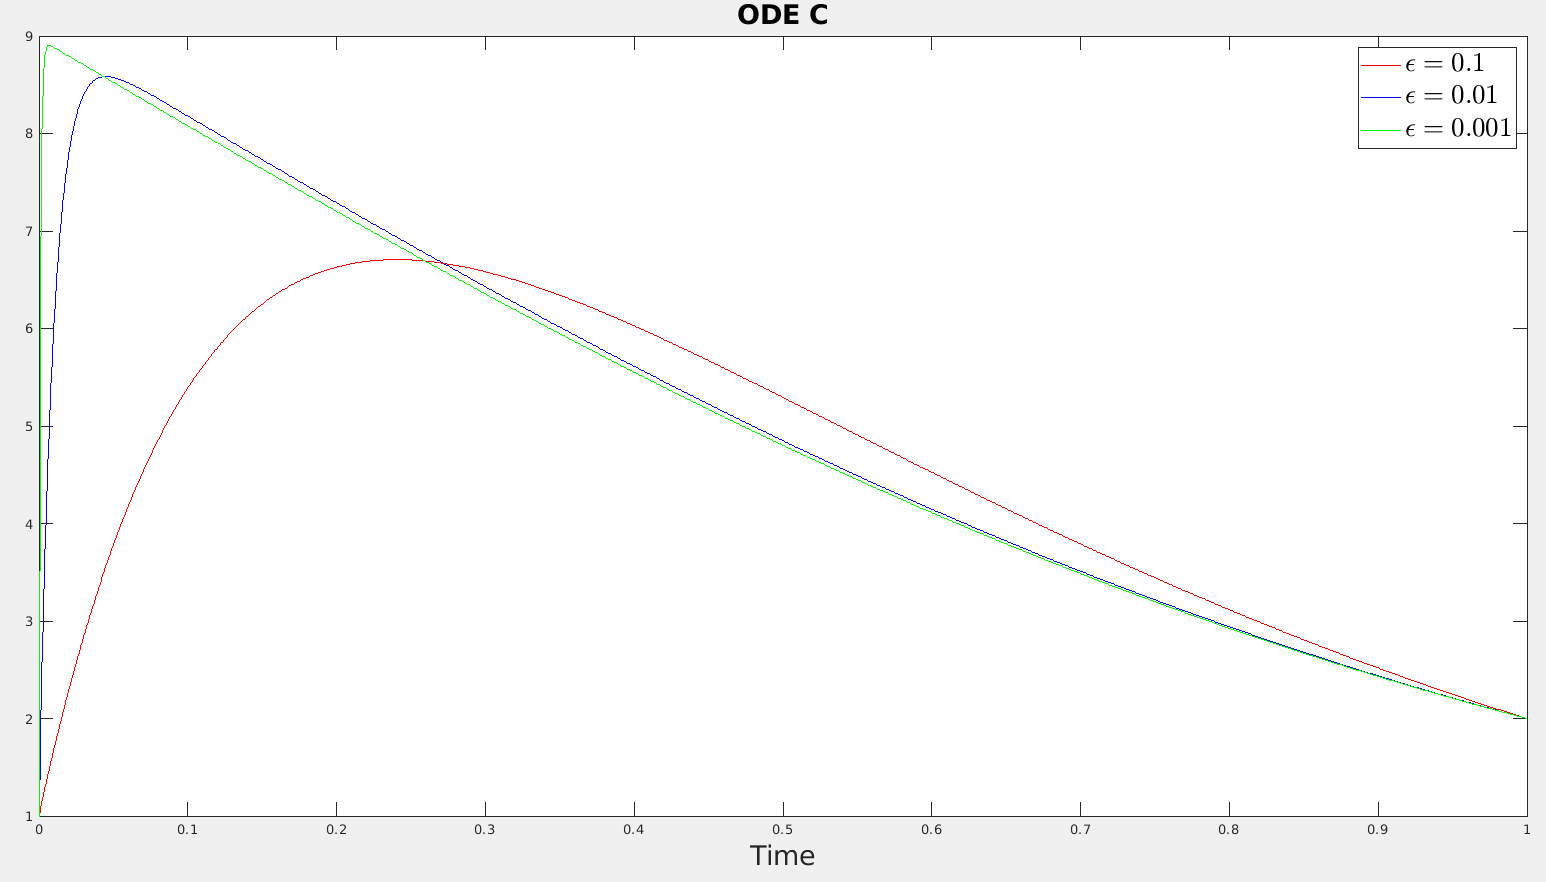
\includegraphics[width=.8\textwidth]{images/ODEC.png}
            \caption{Numerical Solution for differing $\epsilon$ obtained using
            the shooting method and `ode45'}
            \label{fig:ODEC_num_sol}
        \end{figure}
    \item For this problem, I will use the Boundary Layer method as this PDE has
    2 (Boundary) conditions as well as the fact that the second order term in
    the ODE disappears as $\epsilon \to 0$ creating a Boundary Layer problem.
    \item First we find the outer solution by setting $\epsilon = 0$, 
    \begin{gather*}
        \frac{df_{out}}{dt} = - (t+1)f_{out}, \quad f(1) = 2\\
        \frac{df_{out}}{f} = - (t+1)dt\\
        \ln|f_{out}| = -\frac{t^2}{2} - t + c\\
        f_{out}(t) = Ce^{-t^2/2 - t}\\
        \textbf{IC} \to f_{out}(t) = 2e^{-t^2/2 - t + 3/2}
    \end{gather*}
    This completes the outer solution. Next we must begin the inner solution by
    determining the dominant balance. First we set $t = s\epsilon^{\alpha}$. 

    \bmp{.47}
        \begin{gather*}
            \epsilon^{1-2\alpha}\frac{d^2f_{in}}{ds^2} \approx
            -\epsilon^{-\alpha}\frac{df_{in}}{ds} \\
            f_{in} = O(1) \implies \alpha = 1\\
            (s\epsilon + 1)f_{in} \ll O(\epsilon^{-1})
        \end{gather*}
        This method is self-consistent. 
    \emp
    \bmp{.47}
        \begin{gather*}
            \epsilon^{1-2\alpha}\frac{d^2f_{in}}{ds^2} \approx
            -(se^{\alpha} +1)f_{in}\\
            f_{in} = O(1) \implies \alpha = \frac{1}{3}\\
            \epsilon^{-1/3}\frac{df_{in}}{ds} \gg O(\epsilon^{1/3})
        \end{gather*}
        This method is not self consistent; the term it disregards becomes the
        most dominant term in the equation. 
    \emp

    Thus we proceed with $\alpha = 1$ and disregard $(s\epsilon +1)f$ from
    the equation. 

    \begin{gather*}
        \frac{d^2f_{in}}{ds^2} = -\frac{df_{in}}{ds}\\
        \frac{df_{in}}{ds} = c_1e^{-s}\\
        f_{in}(s) = -c_1e^{-s} + c_2\\
        f_{in}(0) = 1 \implies c_1 = 1 - c_2
    \end{gather*}
    From here we proceed with Prandtl's matching condition.
    \begin{gather*}
        \lim_{s\to\infty} f_{in}(s) = \lim_{x\to0} f_{out}(x)\\
        c_2 = 2e^{3/2} \implies c_1 = 1 - 2e^{3/2}\\
        f_{in} = (1 - 2e^{3/2})e^{-t/\epsilon} + 2e^{3/2}
    \end{gather*}
    Finally we write the composite solution. 
    \begin{gather*}
        f = f_{in} + f_{out} - L\\
        f = (1 - 2e^{3/2})e^{-t/\epsilon} + 2e^{-t^2/2 - t + 3/2}
    \end{gather*}

    \item As seen in Figure \ref{fig:ODEC_comp}, the asymptotic solution approximates the
    numerical solution very closely. It should be noted that the Boundary Layer
    method often produces some degree of error which qualitatively decreases with
    $\epsilon$. For example, the error for $\epsilon = 0.1$ is quite large,
    however, the error for $\epsilon = 0.001$ is not noticeable to the eye on
    the plot. 
        \begin{figure}
            \centering
            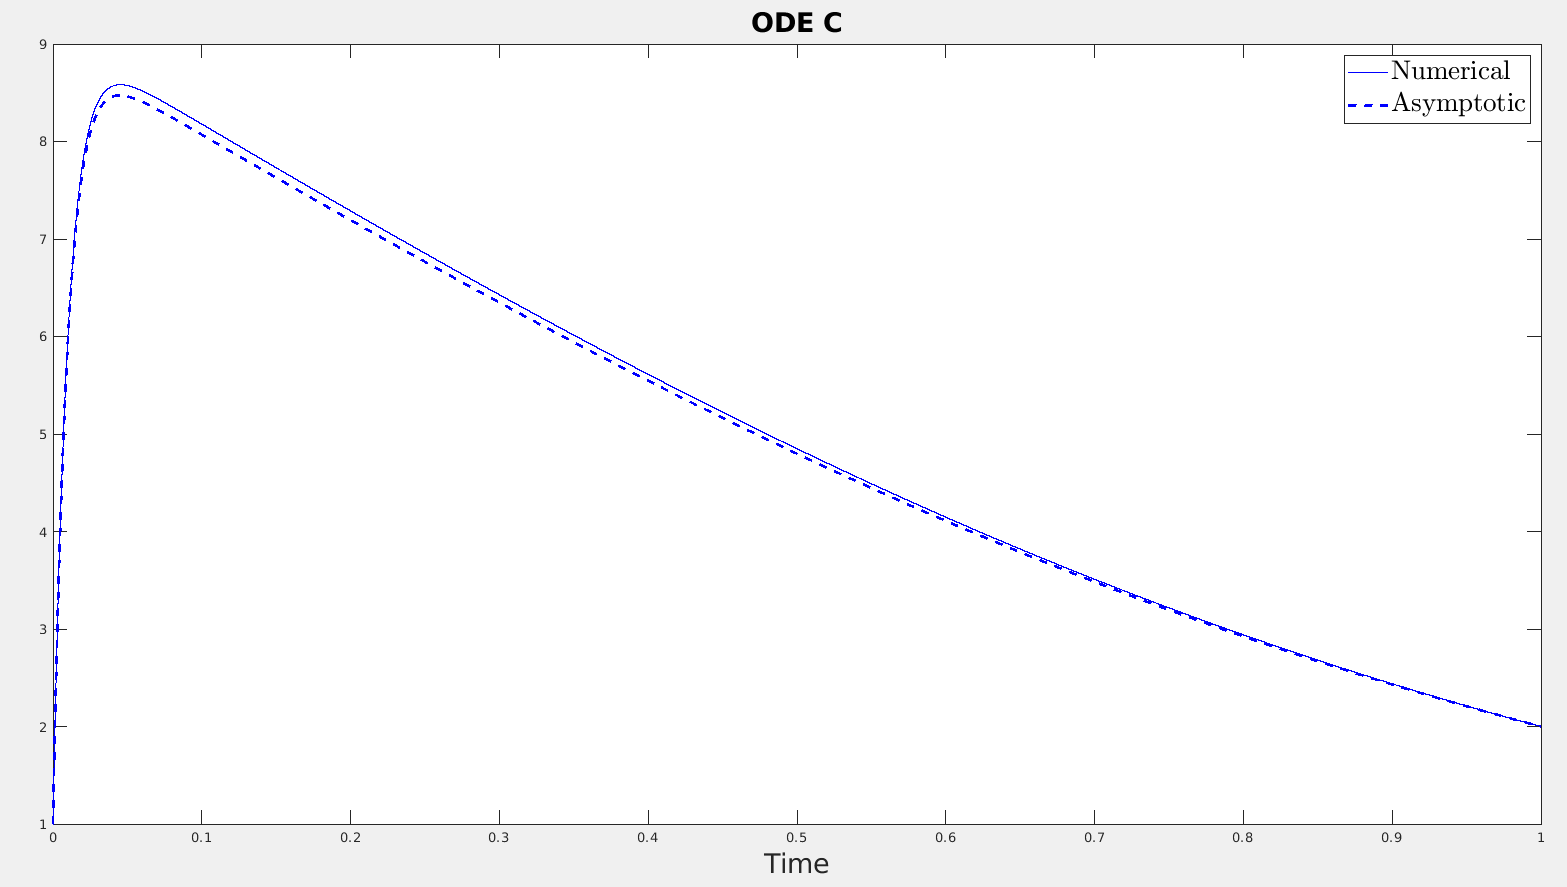
\includegraphics[width=.8\textwidth]{images/ODEC_sol.png}
            \caption{Comparison between numerical and asymptotic solutions for
            $\epsilon = 0.01$}
            \label{fig:ODEC_comp}
        \end{figure}

\end{enumerate}

\vspace{10pt}

\hline

\vspace{10pt}

\section*{Problem 2}
Find the eigenvalues and eigenfunctions of this eigenvalue problem, in the
limite where the eigenvalue $\lambda$ is very large and positive. 

\begin{gather*}
    \frac{d^2f}{dt^2} + \lambda(x+1)^2f = 0 \quad \text{with } f(1) = 0, f(2) =
    0\\
\end{gather*}

We begin solving this proble using WKB theory and following the procedure
described in the notes. First we put this problem in SL form. 
\begin{gather*}
    \frac{d}{dt}\left(\frac{df}{dt}\right) = -\lambda(x+1)^2f, \quad p(x) = 1,
    \quad q(x) = 0, \quad w(x) = (x+1)^2
\end{gather*}
The first step is to take $\lambda = 1/\epsilon^2$ and introduce the WKB
rescaling of $x_f = g(x)/\epsilon$. 

\begin{gather*}
    \left(\frac{\partial}{\partial \ts} + \frac{g'(x_s)}{\epsilon}
    \frac{\partial}{\partial \xf}\right)\left(\frac{\partial f}{\partial \xs} +
    \frac{g'(x_s)}{\epsilon}
    \frac{\partial f}{\partial \xf}\right) = -\frac{(\xs+1)^2}{\epsilon^2}f\\
    O(\epsilon^{-2}): \quad \frac{g'^2(\xs)}{\epsilon^2}\frac{\partial^2 f_0}{\partial \xf^2} = -
    \frac{(\xs+1)^2}{\epsilon^2}f_0 \implies g'(\xs) = (\xs+1)\\
    f_0 = a(\xs)\cos(\xf) + b(\xs)\sin(xf), \quad g(x_s) = \frac{\xs^2}{2} + \xs
    - \frac{3}{2}\\
    O(\epsilon^{-1}): \quad 2(x+1)\frac{\partial^2 f_0}{\partial
    \xs\partial\xf} + \frac{\partial f}{\partial xf} +
    (\xs+1)^2 \frac{\partial^2f_1}{\partial xf^2} = 
    - (\xs+1)^2f_1\\
    2(\xs+1)\left(-a'(\xs)\sin(\xf) + b'(\xs)\cos(\xf)\right) +
    \left(-a(\xs)\sin(\xf) + b(\xs)\cos(\xf)\right) +
    (\xs+1)^2\frac{\partial^2f_1}{\partial \xf^2} = -(\xs+1)^2f_1
\end{gather*}
We have sources of secular terms in this equation and in order to eliminate
those terms we require the following equations hold:

\bmp{.49}
    \begin{gather*}
        2(\xs+1)a'(\xs) = -a(\xs)\\
        a'(\xs) = -\frac{a(\xs)}{2(\xs+1)}\\
        \frac{da}{a} = -\frac{\xs}{2(\xs+1)}\\
        \ln|a| = -\frac{1}{2}\ln|\xs+1| + c\\
        a = A(\xs+1)^{-1/2}
    \end{gather*}
\emp
\bmp{.49}
    \begin{gather*}
        2(\xs+1)b'(\xs) = -b(\xs)\\
        b'(\xs) = -\frac{b(\xs)}{2(x+1)}\\
        \frac{db}{b} = -\frac{\xs}{2(\xs+1)}\\
        \ln|b| = -\frac{1}{2}\ln|\xs+1| + c\\
        b = B(\xs+1)^{-1/2}
    \end{gather*}
\emp

Thus we have 

\begin{gather*}
    f_0 = v_n = (x+1)^{-1/2}\left(A\cos\left(\frac{x^2/2 + x - 3/2}{\epsilon}\right) +
    B\sin\left(\frac{x^2/2 + x - 3/2}{\epsilon}\right)\right)\\
    \textbf{BC} \to A = 0, \quad \epsilon = \frac{5}{2n\pi}\\
    \lambda_n = \frac{4n^2\pi^2}{25}
\end{gather*}
For this problem we can approximate the eigenfunctions $v_n$ with $f_0$ and the
corresponding eigenvalue with $\lambda_n$ when the eigenvalues are very large. 

\end{document}


